\subsection{Caso d'uso UC3: Modifica presentazione}
\begin{figure}[h] 
	\centering 
	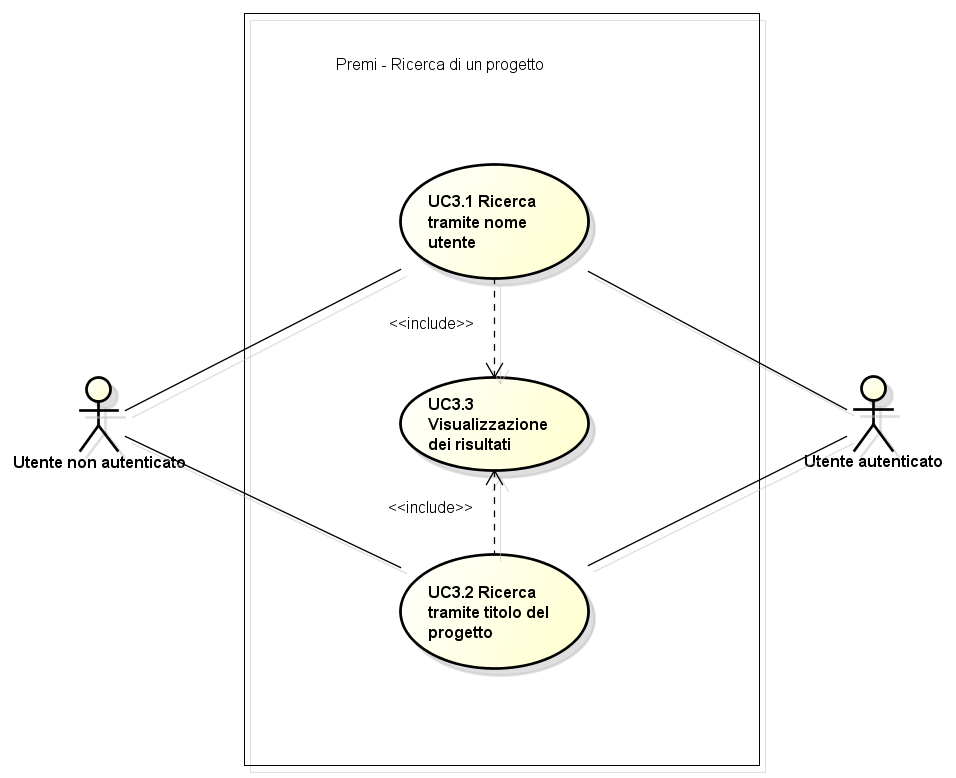
\includegraphics[scale=0.45] {img/UC3.png} 
	\caption{UC3 - Modifica presentazione} 
\end{figure}

\begin{itemize}
	\item \textbf{Attori:} Utente;
	\item \textbf{Scopo e descrizione:} L'utente può selezionare una slide della presentazione e poi un suo elemento al fine di modificarne il contenuto, oppure può inserire del nuovo contenuto;
	\item \textbf{Precondizione:} Nel sistema è già caricata una presentazione e viene mostrata la schermata di creazione di una presentazione con tutte le slide create. L'utente vuole apportare alcune modifiche ad una o più slide;
	\item \textbf{Flusso degli eventi:}
	\begin{enumerate}
		\item L'utente seleziona una slide [UC3.1];
		\item L'utente seleziona un elemento della slide da modificare [UC3.2];
		\item L'utente modifica l'elemento [UC3.3];
		\item L'utente può inserire nuovi elementi nella slide [UC3.4].
	\end{enumerate}
	\item \textbf{Postcondizione:} Il sistema mostra le modifiche effettuate dall'utente sulle slide modificate.
\end{itemize}

\subsection{Caso d'uso UC3.1: Selezione della slide}
\begin{itemize}
	\item \textbf{Attori:} Utente;
	\item \textbf{Scopo e descrizione:} L'utente seleziona dalla lista delle slide della presentazione quelle che intende modificare;
	\item \textbf{Precondizione:} Il sistema mostra tutte le slide della presentazione;
	\item \textbf{Postcondizione:} Il sistema mostra la slide selezionata dall'utente.
\end{itemize}

\subsection{Caso d'uso UC3.2: Selezione di un elemento della slide}
\begin{itemize}
	\item \textbf{Attori:} Utente;
	\item \textbf{Scopo e descrizione:} L'utente seleziona l'elemento della slide che intende modificare;
	\item \textbf{Precondizione:} Il sistema mostra tutti gli elementi contenuti nella slide;
	\item \textbf{Postcondizione:} Il sistema seleziona l'elemento scelto dall'utente.
\end{itemize}


\subsection{Caso d'uso UC3.3: Modifica elemento}
\begin{figure}[h] 
	\centering 
	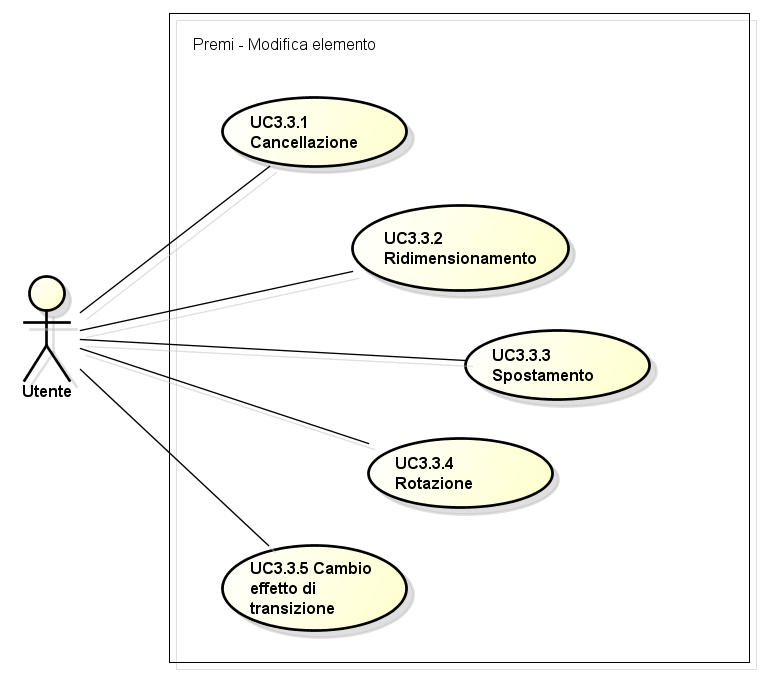
\includegraphics[scale=0.45] {img/UC3.3.png} 
	\caption{UC3.3 - Modifica elemento} 
\end{figure}

\begin{itemize}
	\item \textbf{Attori:} Utente;
	\item \textbf{Scopo e descrizione:} L'utente può modificare in vari modi l'elemento selezionato;
	\item \textbf{Precondizione:} Il sistema presenta un elemento selezionato nella slide;
	\item \textbf{Flusso degli eventi:}
	\begin{enumerate}
		\item L'utente può cancellare l'elemento [UC3.3.1];
		\item L'utente può cambiare dimensione all'elemento [UC3.3.2];
		\item L'utente può cambiare posizione all'elemento [UC3.3.3];
		\item L'utente può ruotare l'elemento [UC3.3.4];
		\item L'utente può cambiare l'effetto di transizione della slide
	\end{enumerate}
	\item \textbf{Postcondizione:} Il sistema ha modificato l'elemento della slide secondo le scelte fatte dall'utente.
\end{itemize}

\subsection{Caso d'uso UC3.3.1: Cancellazione}
\begin{itemize}
	\item \textbf{Attori:} Utente;
	\item \textbf{Scopo e descrizione:} L'utente elimina un elemento selezionato dalla slide;
	\item \textbf{Precondizione:} Il sistema mostra l'elemento selezionato che si intende cancellare;
	\item \textbf{Postcondizione:} Il sistema ha cancellato l'elemento dalla slide.
\end{itemize}

\subsection{Caso d'uso UC3.3.2: Ridimensionamento}
\begin{itemize}
	\item \textbf{Attori:} Utente;
	\item \textbf{Scopo e descrizione:} L'utente cambia grandezza ad un elemento della slide;
	\item \textbf{Precondizione:} Il sistema mostra l'elemento selezionato che si intende ridimensionare;
	\item \textbf{Postcondizione:} Il sistema ha ridimensionato l'elemento della slide.
\end{itemize}

\subsection{Caso d'uso UC3.3.3: Spostamento}
\begin{itemize}
	\item \textbf{Attori:} Utente;
	\item \textbf{Scopo e descrizione:} L'utente cambia di posizione un elemento della slide;
	\item \textbf{Precondizione:} Il sistema mostra l'elemento selezionato che si intende spostare;
	\item \textbf{Postcondizione:} Il sistema ha spostato l'elemento della slide.
\end{itemize}

\subsection{Caso d'uso UC3.3.4: Rotazione}
\begin{itemize}
	\item \textbf{Attori:} Utente;
	\item \textbf{Scopo e descrizione:} L'utente ruota un elemento della slide;
	\item \textbf{Precondizione:} Il sistema mostra l'elemento selezionato che si intende ruotare;
	\item \textbf{Postcondizione:} Il sistema ha ruotato l'elemento della slide.
\end{itemize}

\subsection{Caso d'uso UC3.3.5: Cambio effetto di transizione}
\begin{itemize}
	\item \textbf{Attori:} Utente;
	\item \textbf{Scopo e descrizione:} L'utente cambia l'effetto di transizione della slide corrente;
	\item \textbf{Precondizione:} Il sistema mostra la slide alla quale si intende modificare l'effetto di transizione;
	\item \textbf{Postcondizione:} Il sistema ha cambiato l'effetto di transizione della slide.
\end{itemize}
\newpage

\subsection{Caso d'uso UC3.4: Inserimento nuovo contenuto}

\begin{figure}[h] 
	\centering 
	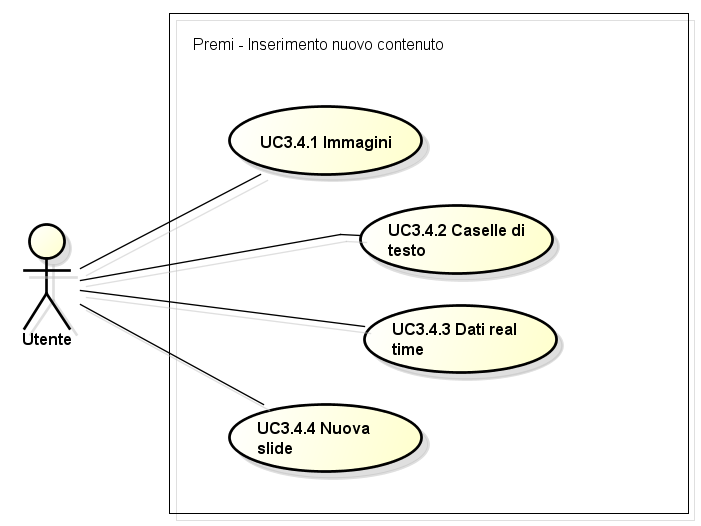
\includegraphics[scale=0.45] {img/UC3.4.png} 
	\caption{UC3.4 - Inserimento nuovo contenuto} 
\end{figure}


\begin{itemize}
	\item \textbf{Attori:} Utente;
	\item \textbf{Scopo e descrizione:} L'utente può inserire del nuovo contenuto all'interno della slide oppure aggiungere una nuova slide da inserire dopo quella attualmente selezionata;
	\item \textbf{Precondizione:} Il sistema mostra la slide selezionata;
	\item \textbf{Flusso degli eventi:}
	\begin{enumerate}
		\item L'utente può inserire immagini [UC3.4.1];
		\item L'utente può inserire caselle di testo [UC3.4.2];
		\item L'utente può inserire dati \gls{real time} [UC3.4.3];
		\item L'utente può inserire una nuova slide [UC3.4.4].
	\end{enumerate}
	\item \textbf{Postcondizione:} Il sistema mostra i nuovi elementi inseriti dall'utente nella slide selezionata.
\end{itemize}


\subsection{Caso d'uso UC3.4.1: Immagini}
\begin{itemize}
	\item \textbf{Attori:} Utente;
	\item \textbf{Scopo e descrizione:} L'utente inserisce un'immagine nella slide corrente;
	\item \textbf{Precondizione:} Il sistema mostra la slide nella quale si vuole inserire la nuova immagine;
	\item \textbf{Postcondizione:} Il sistema ha inserito l'immagine nella slide.
\end{itemize}

\subsection{Caso d'uso UC3.4.2: Caselle di testo}
\begin{itemize}
	\item \textbf{Attori:} Utente;
	\item \textbf{Scopo e descrizione:} L'utente inserisce una casella di testo nella slide corrente;
	\item \textbf{Precondizione:} Il sistema mostra la slide nella quale si vuole inserire la casella di testo;
	\item \textbf{Postcondizione:} Il sistema ha inserito la casella di testo nella slide.
\end{itemize}

\subsection{Caso d'uso UC3.4.3: Dati real time}
\begin{itemize}
	\item \textbf{Attori:} Utente;
	\item \textbf{Scopo e descrizione:} L'utente inserisce dei dati \gls{real time} nella slide corrente;
	\item \textbf{Precondizione:} Il sistema mostra la slide nella quale si vogliono inserire i dati \gls{real time};
	\item \textbf{Postcondizione:} Il sistema ha inserito i dati \gls{real time} nella slide.
\end{itemize}

\subsection{Caso d'uso UC3.4.1: Nuova slide}
\begin{itemize}
	\item \textbf{Attori:} Utente;
	\item \textbf{Scopo e descrizione:} L'utente inserisce una nuova slide vuota dopo quella selezionata;
	\item \textbf{Precondizione:} Il sistema mostra la slide selezionata;
	\item \textbf{Postcondizione:} Il sistema ha inserito una nuova slide vuota dopo la slide selezionata.
\end{itemize}